\section{Основная часть}
    \subsection{Постановка задачи}
        Пусть дана система линейных алгебраических уравнений. Представим её таким образом: известные квадратная матрица $A$, вектор $f$ и неизвестный вектор $x$ размерностями $n$. Нужно найти вектор $x$ в матричном уравнении $Ax = f$, используя метод отражений.
        
    \subsection{Описание алгоритма}
        Метод отражений состоит в выполнении $(n-1)$ шагов, в результате чего матрица $A$ приводится к верхней треугольной форме и в последующей решении системы с такой матрицей.

        Для этого на каждом шаге $k$ будем находить вектор нормали $p$, характеризующий ортогональную матрицу отражения $P$, которая обнулит все поддиагональные элементы $k$-того столбца.

        Обозначим вектор нормали и матрицу на шаге $k$: $p^{(k)}, A_{k} = \left( a_{ij}^{(k)} \right)$, тогда
        \[
            p_k^{(k)} = a_{kk}^{(k-1)} + \sigma_k \sqrt{\sum_{l=k}^{n} \left( a_{lk}^{(k-1)} \right)^2 }, \quad \sigma_k = \left\{
                \begin{matrix}
                    1, & a_{kk}^{(k-1)} \geq 0, \\
                    -1, & a_{kk}^{(k-1)} \leq 0,
                \end{matrix}
            \right.
        \]
        \[
            p_i^{(k)} = 0, \quad i = 0, \dots, k - 1; \qquad p_i^{(k)} = a_{ik}^{(k-1)} , \quad i = k+1, \dots, n;
        \]
        Определение матрицы $ P_k = I - \frac{2 p^{(k)} \left(p^{(k)}\right)^*}{(p^{(k)},p^{(k)})}$. Будем применять данную матрицу с обоих сторон уравнения. Связь шагов $ A_k = P_k A_{k-1},~ f^{(k)} = P_k f^{(k-1)} $. 
        
        Запишем явные формулы элементов матрицы $ A_k $ и вектора $ f^{(k)} $:
        
        \[
            \begin{split}
                a_{kk}^{(k)} = - \sigma_k \sqrt{\sum_{l=k}^{n} \left( a_{lk}^{(k-1)} \right)^2 }, \quad
                a_{ij}^{(k)} = a_{ij}^{(k-1)} - 2 p_i^{(k)} ~\frac{\sum\limits_{l=k}^{n} \left( p_l^{(k)} a_{lj}^{(k-1)} \right)}{\sum\limits_{l=k}^{n} \left( p_{l}^{(k)} \right)^2}, \\
                f_i^{(k)} = f_i^{(k-1)} - 2 p_i^{(k)} ~\frac{\sum\limits_{l=k}^{n} \left( p_l^{(k)} f_l^{(k-1)} \right)}{\sum\limits_{l=k}^{n} \left( p_{l}^{(k)} \right)^2}; \quad
                i = k, \dots, n, \quad j = k+1, \dots, n.
            \end{split}
        \]

        В результате выполнения всех $(n-1)$ шагов получится система $ A_{n-1} x = f^{(n-1)} $, где матрица $ A_{n-1} $ является верхней треугольной, поэтому вектор $ x $ можно найти последовательно снизу вверх:
        \[
            x_n = \frac{ f_n^{(n-1)} }{ a_{nn}^{(n-1)} }, \quad x_i = \frac{ f_i^{(n-1)} - \sum\limits_{j=i+1}^n a_{ij}^{(n-1)} x_j  }{ a_{ii}^{(n-1)} }, \quad
            i = n-1, \dots, 1.
        \]

    
        Сложность данного алгоритма $O(n^3)$. Это оценка основывается на том, что на для вычисления сумм требуется в среднем $ \frac{n}{2} $, при этом такие суммы рассчитываются на каждом для каждого элемента, выше диагонали, что можно оценить как $ \frac{n^2}{2} $.

    
    \subsubsection{Погрешности вычислений}
        Данный метод является точным численным методом, поэтому погрешность вычислений зависит от погрешности представления числа в компьютере и количестве проделанных операций деления. Из этого следует, что, используя более точные типы данных, результат будет более точный.


    \subsection{Вычислительные эксперименты}
        Для вычислительных экспериментов будут использованы матрицы и вектора, предложенные на практических занятиях по вычислительной математике, из пособия[\ref{3.15}], а также несколько специально подобранных. Матрицы можно найти в секции <<\nameref{appendices}>>.

        В таблице \ref{res-tab} приведены модули максимальных погрешностей:
        \begin{itemize}
            \item $ \Delta(x) $ -- по найденному вектору $ x $ и решению, полученному встроенной функции пакета <<numpy>>.
            \item $ \Delta(f) $ -- по вычисленному вектору $ Ax $ и данному вектору $ f $.
        \end{itemize}

        \begin{table}[H]            
            \begin{center}
                \begin{tabular}{| c | c | c | c |}
                    \hline
                    № данных & $ \mu(A) $ & $ \Delta(x) $ & $ \Delta(f) $ \\ \hline
                    \ref{matrix1} & 7.3257 & 2.22e-16 & 4.44e-16 \\ \hline
                    \ref{matrix2} & 660.085 & 2.13e-14 & 1.42e-14 \\ \hline
                    \ref{matrix3} & 954.552 & 1.37e-14 & 9.77e-15 \\ \hline
                    \ref{matrix4} & 220.045 & 5.3e-15 & 1.69e-15 \\ \hline
                    \ref{matrix5} & 20001 & 1.57e-12 & 4.44e-16 \\ \hline
                    \ref{matrix6} & 20000001 & 1.57e-09 & 4.44e-16 \\ \hline
                \end{tabular}
                \caption{\label{res-tab}Таблица результатов.}
            \end{center}
        \end{table}

        \subsubsection{Анализ результатов}
            Как можно увидеть, погрешность увеличивается с увеличением числа обусловленности, потому что число обусловленности показывает насколько сильно небольшое изменение в правой части уравнения ведёт к изменению в решении.

            Погрешность в получаемом векторе $ Ax $ во всех экспериментах была достаточно близка, и можно сделать вывод, что число обусловленности на него в данных экспериментах не влияет.




% \begin{figure}[H]
%     \centering
%     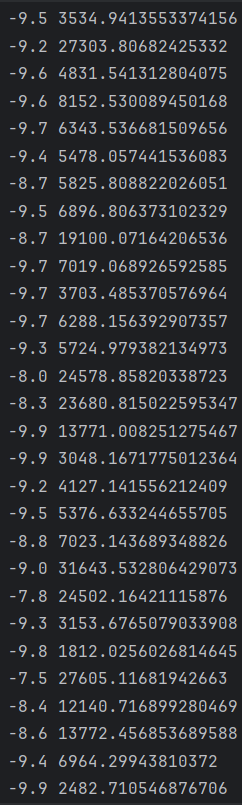
\includegraphics[width=6cm]{pictures/BigConditions.png}
%     \caption{Log10 разности и число обусловленности решений, которые не превысили точность $10^{-10}$.}
% \end{figure}